\begin{figure}[tb]
  \centering
  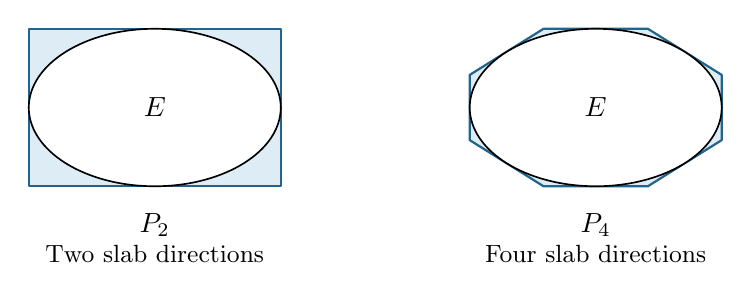
\begin{tikzpicture}[x=1cm,y=1cm,line join=round]
    \definecolor{slabblue}{RGB}{34,100,139}
    \definecolor{slabfill}{RGB}{222,237,245}
    \begin{scope}[xshift=-2.8cm]
      \filldraw[fill=slabfill,draw=slabblue,line width=0.8pt]
        (-1.6,-1) rectangle (1.6,1);
      \filldraw[fill=white,draw=black,line width=0.6pt]
        (0,0) ellipse [x radius=1.6,y radius=1];
      \node at (0,0) {$E$};
      \node[anchor=north] at (0,-1.22) {$P_2$};
      \node[anchor=north,font=\small] at (0,-1.62)
        {Two slab directions};
    \end{scope}
    \begin{scope}[xshift=2.8cm]
      \foreach \k in {0,...,7} {
        \coordinate (p\k) at
          ({1.6*cos(22.5+45*\k)/cos(22.5)},
           {sin(22.5+45*\k)/cos(22.5)});
      }
      \filldraw[fill=slabfill,draw=slabblue,line width=0.8pt]
        (p0) \foreach \k in {1,...,7} {-- (p\k)} -- cycle;
      \filldraw[fill=white,draw=black,line width=0.6pt]
        (0,0) ellipse [x radius=1.6,y radius=1];
      \node at (0,0) {$E$};
      \node[anchor=north] at (0,-1.22) {$P_4$};
      \node[anchor=north,font=\small] at (0,-1.62)
        {Four slab directions};
    \end{scope}
  \end{tikzpicture}
  \caption{Finite outer approximations of an ellipse $E$. Adding slab
  directions gives $P_2\supset P_4\supset E$; the subscripts here count
  slab directions. Using nested finite spanning direction
  sets with dense union, the same construction recovers $\mathcal W[f]$ from any
  positive continuous even function $f$ on the sphere; $f$ need not be a
  support function.}
  \label{fig:slab-exhaustion}
\end{figure}
